
\documentclass[letterpaper,hide notes,xcolor={table,svgnames},pdftex,10pt]{beamer}
\def\showexamples{t}

\usecolortheme{crane}
\setbeamertemplate{navigation symbols}{}

\usetheme{MyPittsburgh}
\usepackage{hyperref}
\usepackage{graphicx,xspace}
\usepackage[normalem]{ulem}
\usepackage{multicol}
\usepackage{amsmath,amssymb,amsthm,graphicx,xspace}
\newcommand\SF[1]{$\bigstar$\footnote{SF: #1}}

\usepackage[sfdefault,lf]{carlito}
\usepackage[T1]{fontenc}
\usepackage[scaled]{beramono}
\usepackage{tikzpagenodes}
\newcommand{\Rplus}{\protect\hspace{-.1em}\protect\raisebox{.35ex}{\small{\small\textbf{+}}}}
\newcommand{\Cpp}{\mbox{C\Rplus\Rplus}\xspace}

\newcounter{tmpnumSlide}
\newcounter{tmpnumNote}

\newcommand\mnote[1]{%
	\addtocounter{tmpnumSlide}{1}
	\ifdefined\showcues {~\tiny\fbox{\arabic{tmpnumSlide}}}\fi
	\note{\setlength{\parskip}{1ex}\addtocounter{tmpnumNote}{1}\textbf{\Large \arabic{tmpnumNote}:} {#1\par}}}

\newcommand\mmnote[1]{\note{\setlength{\parskip}{1ex}#1\par}}


\newcommand\mquestion[2]{{~\color{red}\fbox{?}}\note{\setlength{\parskip}{1ex}\par{\Large \textbf{?}} #1} \note{\setlength{\parskip}{1ex}\par{\Large \textbf{A}} #2\par}\ifdefined \presentationonly \pause \fi}

\newcommand\blackboard[1]{%
	\ifdefined   \showblackboard
		{#1}
	\else {\begin{center} \fbox{\colorbox{blue!30}{%
						\begin{minipage}{.95\linewidth}%
							\hspace{\stretch{1}} Some space intentionally left blank; done at the blackboard.%
						\end{minipage}}}\end{center}}%
	\fi%
}

\usepackage{listings}
\lstset{%
	keywordstyle=\bfseries,
	aboveskip=15pt,
	belowskip=15pt,
	captionpos=b,
	identifierstyle=\ttfamily,
	frame=lines,
	numbers=left, basicstyle=\scriptsize, numberstyle=\tiny, stepnumber=0, numbersep=2pt}

\usepackage{siunitx}
\newcommand\sius[1]{\num[group-separator = {,}]{#1}\si{\micro\second}}
\newcommand\sims[1]{\num[group-separator = {,}]{#1}\si{\milli\second}}
\newcommand\sins[1]{\num[group-separator = {,}]{#1}\si{\nano\second}}
\sisetup{group-separator = {,}, group-digits = true}

%% -------------------- tikz --------------------
\usepackage{tikz}
\usetikzlibrary{positioning}
\usetikzlibrary{arrows,backgrounds,automata,decorations.shapes,decorations.pathmorphing,decorations.markings,decorations.text}

\tikzstyle{place}=[circle,draw=blue!50,fill=blue!20,thick, inner sep=0pt,minimum size=6mm]
\tikzstyle{transition}=[rectangle,draw=black!50,fill=black!20,thick, inner sep=0pt,minimum size=4mm]

\tikzstyle{block}=[rectangle,draw=black, thick, inner sep=5pt]
\tikzstyle{bullet}=[circle,draw=black, fill=black, thin, inner sep=2pt]

\tikzstyle{pre}=[<-,shorten <=1pt,>=stealth',semithick]
\tikzstyle{post}=[->,shorten >=1pt,>=stealth',semithick]
\tikzstyle{bi}=[<->,shorten >=1pt,shorten <=1pt, >=stealth',semithick]

\tikzstyle{mut}=[-,>=stealth',semithick]

\tikzstyle{treereset}=[dashed,->, shorten >=1pt,>=stealth',thin]

\usepackage{ifmtarg}
\usepackage{xifthen}
\makeatletter
% new counter to now which frame it is within the sequence
\newcounter{multiframecounter}
% initialize buffer for previously used frame title
\gdef\lastframetitle{\textit{undefined}}
% new environment for a multi-frame
\newenvironment{multiframe}[1][]{%
	\ifthenelse{\isempty{#1}}{%
		% if no frame title was set via optional parameter,
		% only increase sequence counter by 1
		\addtocounter{multiframecounter}{1}%
	}{%
		% new frame title has been provided, thus
		% reset sequence counter to 1 and buffer frame title for later use
		\setcounter{multiframecounter}{1}%
		\gdef\lastframetitle{#1}%
	}%
	% start conventional frame environment and
	% automatically set frame title followed by sequence counter
	\begin{frame}%
		\frametitle{\lastframetitle~{\normalfont(\arabic{multiframecounter})}}%
		}{%
	\end{frame}%
}
\makeatother

\makeatletter
\newdimen\tu@tmpa%
\newdimen\ydiffl%
\newdimen\xdiffl%
\newcommand\ydiff[2]{%
	\coordinate (tmpnamea) at (#1);%
	\coordinate (tmpnameb) at (#2);%
	\pgfextracty{\tu@tmpa}{\pgfpointanchor{tmpnamea}{center}}%
	\pgfextracty{\ydiffl}{\pgfpointanchor{tmpnameb}{center}}%
	\advance\ydiffl by -\tu@tmpa%
}
\newcommand\xdiff[2]{%
	\coordinate (tmpnamea) at (#1);%
	\coordinate (tmpnameb) at (#2);%
	\pgfextractx{\tu@tmpa}{\pgfpointanchor{tmpnamea}{center}}%
	\pgfextractx{\xdiffl}{\pgfpointanchor{tmpnameb}{center}}%
	\advance\xdiffl by -\tu@tmpa%
}
\makeatother
\newcommand{\copyrightbox}[3][r]{%
	\begin{tikzpicture}%
		\node[inner sep=0pt,minimum size=2em](ciimage){#2};
		\usefont{OT1}{phv}{n}{n}\fontsize{4}{4}\selectfont
		\ydiff{ciimage.south}{ciimage.north}
		\xdiff{ciimage.west}{ciimage.east}
		\ifthenelse{\equal{#1}{r}}{%
			\node[inner sep=0pt,right=1ex of ciimage.south east,anchor=north west,rotate=90]%
			{\raggedleft\color{black!50}\parbox{\the\ydiffl}{\raggedright{}#3}};%
		}{%
			\ifthenelse{\equal{#1}{l}}{%
				\node[inner sep=0pt,right=1ex of ciimage.south west,anchor=south west,rotate=90]%
				{\raggedleft\color{black!50}\parbox{\the\ydiffl}{\raggedright{}#3}};%
			}{%
				\node[inner sep=0pt,below=1ex of ciimage.south west,anchor=north west]%
				{\raggedleft\color{black!50}\parbox{\the\xdiffl}{\raggedright{}#3}};%
			}
		}
	\end{tikzpicture}
}


%% --------------------

%\usepackage[excludeor]{everyhook}
%\PushPreHook{par}{\setbox0=\lastbox\llap{MUH}}\box0}

%\vspace*{\stretch{1}

%\setbox0=\lastbox \llap{\textbullet\enskip}\box0}

\setlength{\parskip}{\fill}

\newcommand\noskips{\setlength{\parskip}{1ex}}
\newcommand\doskips{\setlength{\parskip}{\fill}}

\newcommand\xx{\par\vspace*{\stretch{1}}\par}
\newcommand\xxs{\par\vspace*{2ex}\par}
\newcommand\tuple[1]{\langle #1 \rangle}
\newcommand\code[1]{{\sf \footnotesize #1}}
\newcommand\ex[1]{\uline{Example:} \ifdefined \presentationonly \pause \fi
	\ifdefined\showexamples#1\xspace\else{\uline{\hspace*{2cm}}}\fi}

\newcommand\ceil[1]{\lceil #1 \rceil}


\AtBeginSection[]
{
	\begin{frame}
		\frametitle{Outline}
		\tableofcontents[currentsection]
	\end{frame}
}



\pgfdeclarelayer{edgelayer}
\pgfdeclarelayer{nodelayer}
\pgfsetlayers{edgelayer,nodelayer,main}

\tikzstyle{none}=[inner sep=0pt]
\tikzstyle{rn}=[circle,fill=Red,draw=Black,line width=0.8 pt]
\tikzstyle{gn}=[circle,fill=Lime,draw=Black,line width=0.8 pt]
\tikzstyle{yn}=[circle,fill=Yellow,draw=Black,line width=0.8 pt]
\tikzstyle{empty}=[circle,fill=White,draw=Black]
\tikzstyle{bw} = [rectangle, draw, fill=blue!20,
text width=4em, text centered, rounded corners, minimum height=2em]

\newcommand{\CcNote}[1]{% longname
	This work is licensed under the \textit{Creative Commons #1 3.0 License}.%
}
\newcommand{\CcImageBy}[1]{%
	\includegraphics[scale=#1]{creative_commons/cc_by_30.pdf}%
}
\newcommand{\CcImageSa}[1]{%
	\includegraphics[scale=#1]{creative_commons/cc_sa_30.pdf}%
}
\newcommand{\CcImageNc}[1]{%
	\includegraphics[scale=#1]{creative_commons/cc_nc_30.pdf}%
}
\newcommand{\CcGroupBySa}[2]{% zoom, gap
	\CcImageBy{#1}\hspace*{#2}\CcImageNc{#1}\hspace*{#2}\CcImageSa{#1}%
}
\newcommand{\CcLongnameByNcSa}{Attribution-NonCommercial-ShareAlike}

\newenvironment{changemargin}[1]{% 
	\begin{list}{}{% 
		\setlength{\topsep}{0pt}% 
		\setlength{\leftmargin}{#1}% 
		\setlength{\rightmargin}{1em}
		\setlength{\listparindent}{\parindent}% 
		\setlength{\itemindent}{\parindent}% 
		      \setlength{\parsep}{\parskip}% 
		      }% 
		\item[]}{\end{list}}



\usepackage{multirow}

\title{Lecture 28 --- The Readers-Writers Problem }

\author{Jeff Zarnett \\ \small \texttt{jzarnett@uwaterloo.ca}}\institute{Department of Electrical and Computer Engineering \\
	University of Waterloo}
\date{\today}


\begin{document}

\begin{frame}
	\titlepage

\end{frame}

\begin{frame}
	\frametitle{Reader/Writer Locks}
	Reads don't interfere with one another so we can let them run in parallel!

	But sometimes writes occur, and nobody can read when this happens.

	\begin{center}
		
\includegraphics[width=0.8\textwidth]{images/groupreading.jpg}
	\end{center}
	\hfill Image Credit: Understood.org
\end{frame}

\begin{frame}
	\frametitle{Reader/Writer Rules}


	\begin{enumerate}
		\item Any number of readers may be in the critical section simultaneously.
		\item Only one writer may be in the critical section (and when it is, no readers are allowed).
	\end{enumerate}


	This is very often how file systems work.

\end{frame}


\begin{frame}
	\frametitle{With Variation}

	This is similar to, but distinct from, the general mutual exclusion problem and the producer-consumer problem.

	Readers do not modify the data (consumers do take things out of the buffer, modifying it).

	If any thread could read or write the shared data structure, we would have to use the general mutual exclusion solution.

	Allowing multiple readers can permit better performance!

	And there are many scenarios where updates are rare but reads are common.

\end{frame}

\begin{frame}
	\frametitle{Readers-Writers Solution 1}
	Let us keep track of the number of readers at any given time with \texttt{readers}.

	We will need a way of protecting this variable from concurrent modifications, so there will have to be a binary semaphore \texttt{mutex}.

	We will also need one further semaphore, \texttt{roomEmpty}.

	A writer has to wait for the room to be empty (i.e., \texttt{wait} on the \texttt{roomEmpty} semaphore) before it can enter.
\end{frame}



\begin{frame}[fragile]
	\frametitle{Readers-Writers Solution 1}

	\begin{multicols}{2}
		\textbf{Writer}
		\begin{verbatim}
	 1. wait( roomEmpty )
	 2. [write data]
	 3. post( roomEmpty )
	 
	 
	 
	 
	 
	 
	 
	 
	 
	 
  \end{verbatim}
		\columnbreak
		\textbf{Reader}
		\begin{verbatim}
	 1. wait( mutex )
	 2. readers++
	 3. if readers == 1
	 4.     wait( roomEmpty )
	 5. end if
	 6. post( mutex )
	 7. [read data]
	 8. wait( mutex )
	 9. readers--
	10. if readers == 0
	11.     post( roomEmpty )
	12. end if
	13. post( mutex )
  \end{verbatim}
	\end{multicols}
	\vspace{-2em}

\end{frame}

\begin{frame}
	\frametitle{Readers-Writers Solution 1 Analysis}

	The first reader that arrives encounters the situation that the room is empty, so it ``locks'' the room (waiting on the \texttt{roomEmpty} semaphore).

	That will prevent writers from entering the room.

	Additional readers do not check if the room is empty; they just proceed to enter.

	When the last reader leaves the room, it indicates that the room is empty (``unlocking it'' to allow a writer in).

\end{frame}

\begin{frame}
	\frametitle{Readers-Writers Solution 1 Analysis}

	This pattern is sometimes called the \alert{light switch}.

	\begin{center}
		
\includegraphics[width=0.6\textwidth]{images/lightswitch.png}
	\end{center}

\end{frame}


\begin{frame}
	\frametitle{Readers-Writers Solution 1 Analysis}

	The reader code has that situation that makes us concerned.\\
	\quad A wait on \texttt{roomEmpty} inside a critical section controlled by \texttt{mutex}.

	With a bit of reasoning, we can convince ourselves that there is no deadlock.

	A reader waits on \texttt{roomEmpty} only if a writer is currently in its critical section.

	As long as the write operation takes finite time, eventually the writer will post the \texttt{roomEmpty} semaphore and the threads can continue.

	Deadlock is not a problem.

\end{frame}


\begin{frame}
	\frametitle{Readers-Writers Solution 1 Analysis}

	There is, however, a second problem that we need to be concerned about.

	Suppose some readers are in the room, and a writer arrives.

	The writer must wait until all the readers have left the room.

	When each of the readers is finished, it exits the room.

	In the meantime, more readers arrive and enter the room.
\end{frame}


\begin{frame}
	\frametitle{Readers-Writers Solution 1 Analysis}

	So even though each reader is in the room for only a finite amount of time, there is never a moment when the room has no readers in it.

	This undesirable situation is not deadlock, because the reader threads are not stuck, but the writer (and any subsequent writers) is (are) going to wait forever.

	This is a situation called \alert{starvation}: a thread never gets a chance to run.


\end{frame}


\begin{frame}
	\frametitle{Starvation}

	Recall criterion 3 of properties we want in any mutual exclusion solution:\\
	\quad It must not be possible for a thread to be delayed indefinitely.

	This problem is just as bad as deadlock in that if it is discovered, it eliminates a proposed solution as an acceptable option.

	Even though starvation might only be an unlikely event.

	We must therefore improve on this solution such that there is no longer the possibility that a writer starves.


\end{frame}


\begin{frame}
	\frametitle{Readers-Writers Solution 2}

	When a writer arrives, any readers should be permitted to finish their read.\\
	\quad No new readers should be allowed to start reading.

	Eventually, all the readers currently in the critical section will finish.

	The writer will get a turn, because the room is empty.

	When the writer is done, all the readers that arrived after the writer will be able to enter.

\end{frame}

\begin{frame}[fragile]
	\frametitle{Readers-Writers Solution 2}
	\begin{multicols}{2}
		\textbf{Writer}
		\begin{verbatim}
	 1. wait( turnstile )
	 2. wait( roomEmpty )
	 3. [write data]
	 4. post( turnstile )
	 5. post( roomEmpty )
	 
	 
	 
	 
	 
	 
	 
	 
	 
	 
  \end{verbatim}
		\columnbreak
		\textbf{Reader}
		\begin{verbatim}
	 1. wait( turnstile )
	 2. post( turnstile )
	 3. wait( mutex )
	 4. readers++
	 5. if readers == 1
	 6.     wait( roomEmpty )
	 7. end if
	 8. post( mutex )
	 9. [read data]
	10. wait( mutex )
	11. readers--
	12. if readers == 0
	13.     post( roomEmpty )
	14. end if
	15. post( mutex )
  \end{verbatim}
	\end{multicols}

\end{frame}


\begin{frame}
	\frametitle{Readers-Writers Solution 2 Analysis}

	Does this solution satisfy our goals of avoidance of deadlock and starvation?

	Starvation is fairly easy to assess: the first attempt at the solution had one scenario leading to starvation and this solution addresses it.

	You should be able to convince yourself that the solution as described cannot starve the writers or readers.


\end{frame}


\begin{frame}
	\frametitle{Readers-Writers Solution 2 Analysis}

	On to deadlock: the reader code is minimally changed from before

	The writer has that dangerous pattern: two waits.

	If the writer is blocked on the \texttt{roomEmpty} semaphore, no readers or writers could advance past the turnstile and no writers.

	If the writer is blocked on that semaphore, there are readers in the room.

	The readers will individually finish and leave (their progress is not impeded).

	So the room will eventually become empty; the writer will be unblocked.


\end{frame}

\begin{frame}
	\frametitle{Readers-Writers Solution 2 Analysis}

	Note that this solution does not give writers any particular priority: when a writer exits it posts on \texttt{turnstile} and that may unblock a reader or a writer.

	If it unblocks a reader, a whole bunch of readers may enter before the next writer is unblocked and locks the turnstile again.

	That may or may not be desirable, depending on the application.

	In any event, it does mean it is possible for readers to proceed even if a writer is queued.

	If there is a need to give writers priority, there are techniques for doing so.
\end{frame}


\begin{frame}
	\frametitle{Business Class Passengers Board in Zone 1}

	\begin{center}
		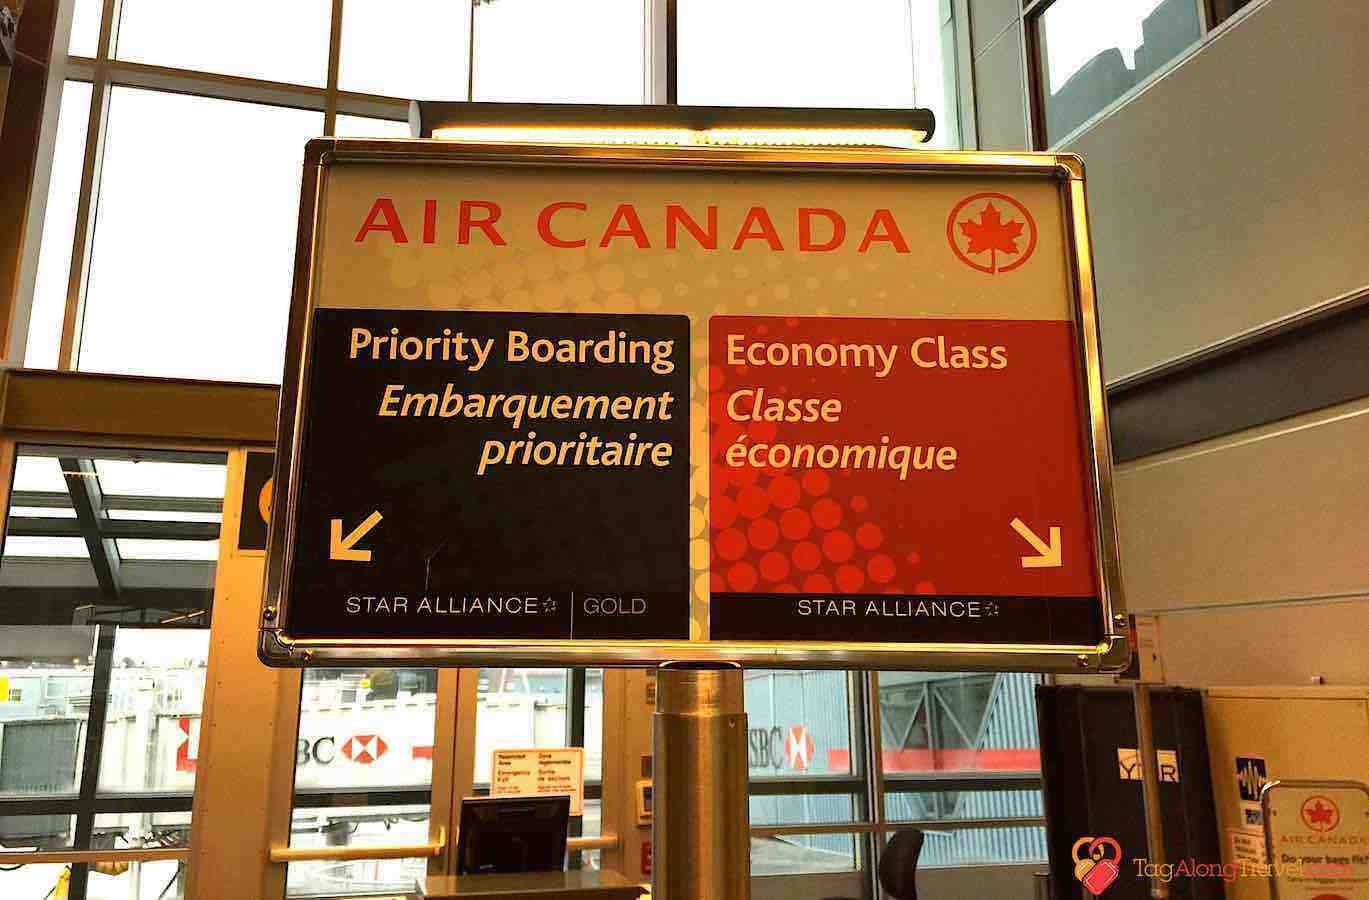
\includegraphics[width=0.9\textwidth]{images/priority-boarding.jpg}
	\end{center}
	\hfill Image Credit: Tag Along Travel
\end{frame}


\begin{frame}
	\frametitle{Business Class Passengers Board in Zone 1}

	Let's modify the solution so that writers have priority over readers.

	We will probably want to break up the \texttt{roomEmpty} semaphore into \texttt{noReaders} and \texttt{noWriters}.

	A reader in the critical section should hold the \texttt{noReaders} semaphore and a writer should hold \texttt{noWriters} and \texttt{noReaders}.

\end{frame}


\begin{frame}[fragile]
	\frametitle{Writer Priority}

	\begin{multicols}{2}
		\textbf{Writer}\vspace{-1em}
		\begin{verbatim}
     1. wait( writeMutex )
     2. writers++
     3. if writers == 1
     4.     wait( noReaders )
     5. end if
     6. post( writeMutex )
     7. wait ( noWriters )
     8. [write data]
     9. post( noWriters ) 
    10. wait( writeMutex )
    11. writers--
    12. if writers == 0
    13.    post( noReaders )
    14. end if
    15. post( writeMutex )     
  \end{verbatim}
		\columnbreak
		\textbf{Reader}\vspace{-2em}
		\begin{verbatim}
     1. wait( noReaders )
     2. wait( readMutex )
     3. readers++
     4. if readers == 1
     5.    wait( noWriters )
     6. end if
     7. post( readMutex )
     8. post( noReaders )
     9. [read data]
    10. wait( readMutex )
    11. readers--
    12. if readers == 0
    13.     post( noWriters )
    14. end if
    15. post( readMutex )
\end{verbatim}
	\end{multicols}
	\vspace{-2em}

\end{frame}


\begin{frame}
	\frametitle{Analysis: Writer Priority}

	Yikes! The complexity for the writer increased dramatically.

	The reader is not all that different than it was before.

	The writer now is to some extent the mirror image of the reader.

\end{frame}


\begin{frame}
	\frametitle{Too Much Typing?}

	Using the pseudocode as above, we can implement the readers-writers behaviour in a given program using only semaphore and mutex constructs.

	But in the pthread library there is support for readers-writers lock types, meaning we don't have to reinvent the wheel.

	The type for the lock is \texttt{pthread\_rwlock\_t}.

\end{frame}


\begin{frame}[fragile]
	\frametitle{RW Lock Syntax: Init, Destroy}

	\begin{lstlisting}[language=C]
pthread_rwlock_init( pthread_rwlock_t * rwlock, pthread_rwlockattr_t * attr )
\end{lstlisting}

	\texttt{rwlock}: the lock to initialize.

	\texttt{attr}: the attributes (\texttt{NULL} for defaults is fine.)


	\begin{lstlisting}[language=C]
pthread_rwlock_destroy( pthread_rwlock_t * rwlock )
\end{lstlisting}

	\texttt{rwlock}: the lock to destroy.


	Both of these are exactly like the regular mutex.

\end{frame}

\begin{frame}[fragile]
	\frametitle{RW Lock Syntax: Locking}

	\begin{lstlisting}[language=C]
pthread_rwlock_rdlock( pthread_rwlock_t * rwlock )
pthread_rwlock_tryrdlock( pthread_rwlock_t * rwlock )
pthread_rwlock_wrlock( pthread_rwlock_t * rwlock )
pthread_rwlock_trywrlock( pthread_rwlock_t  *  rwlock )
\end{lstlisting}

	We can acquire a read lock, or a write lock.

	Pretty self-explanatory, which is which and when you use what.

	For each of those there is an associated trylock function.

	All four functions take one argument: \texttt{rwlock}, the lock.


\end{frame}


\begin{frame}[fragile]
	\frametitle{RW Lock Syntax: Unlock}

	\begin{lstlisting}[language=C]
pthread_rwlock_unlock( pthread_rwlock_t * rwlock )
\end{lstlisting}

	Unlock works just like the regular mutex unlock.

	We do not need to specify what kind of lock we are releasing.

\end{frame}


\begin{frame}
	\frametitle{Writer Priority?}

	As for whether readers or writers get priority, the specification says this is implementation defined.

	If possible, for threads of equal priority, a writer takes precedence over a reader.

	But your system may vary.


\end{frame}



\begin{frame}
	\frametitle{Mine, Mine, Mine!}

	In theory, the same thread may lock the same rwlock $n$ times.

	Just remember to unlock it $n$ times as well.

	Readers get priority? Implementation defined.

\end{frame}


\begin{frame}[fragile]
	\frametitle{Without RW Locks}

	\begin{multicols}{2}
		\begin{lstlisting}[language=C]
int readers;
pthread_mutex_t mutex;
sem_t roomEmpty;

void init( ) {
  readers = 0;
  pthread_mutex_init( &mutex, NULL );
  sem_init( &roomEmpty, 0, 1 );
}

void cleanup( ) {
  pthread_mutex_destroy( &mutex );
  sem_destroy( &roomEmpty );
}
\end{lstlisting}

		\columnbreak

		\begin{lstlisting}[language=C]
void* writer( void* arg ) {
  sem_wait( &roomEmpty );
  write_data( arg );
  sem_post( &roomEmpty );
}

void* reader( void* read ) {
  pthread_mutex_lock( &mutex );
  readers++;
  if ( readers == 1 ) {
    sem_wait( &roomEmpty );
  }
  pthread_mutex_unlock( &mutex );
  read_data( arg );
  pthread_mutex_lock( &mutex );
  readers--;
  if ( readers == 0 ) {
    sem_post( &roomEmpty );
  }
  pthread_mutex_unlock( &mutex );
}
\end{lstlisting}

	\end{multicols}


\end{frame}


\begin{frame}[fragile]
	\frametitle{With RW Locks}

	\begin{multicols}{2}
		\begin{lstlisting}[language=C]
pthread_rwlock_t rwlock;

void init( ) {
  pthread_rwlock_init( &rwlock, NULL );
}

void cleanup( ) {
  pthread_rwlock_destroy( &rwlock );
}
\end{lstlisting}

		\columnbreak

		\begin{lstlisting}[language=C]
void* writer( void* arg ) {
  pthread_rwlock_wrlock( &rwlock );
  write_data( arg );
  pthread_rwlock_unlock( &rwlock );
}

void* reader( void* read ) {
  pthread_rwlock_rdlock( &rwlock );
  read_data( arg );
  pthread_rwlock_unlock( &rwlock );
}
\end{lstlisting}

	\end{multicols}

	Conclusion: don't reinvent the wheel!

\end{frame}


\begin{frame}
	\frametitle{Seek and Destroy}

	\begin{center}
		
\includegraphics[width=0.5\textwidth]{images/seek-and-destroy.jpg}
	\end{center}
	An extension of the readers-writers problem: the search-insert-delete problem.

	Three kinds of thread: searcher, inserter, deleter.

\end{frame}


\begin{frame}
	\frametitle{Searcher Rules}

	\alert{Searchers} merely examine the list; hence they can execute concurrently with each other.

	Searcher threads must call \texttt{void search( void* target )} where the argument to the searcher thread is the element to be found.

	These most closely resemble readers in the readers-writers problem.

\end{frame}

\begin{frame}
	\frametitle{Inserter Rules}

	\alert{Inserters} add new items to the end of the list; only one insertion may take place at a time.

	However, one insert can proceed in parallel with any number of searches.

	Inserter threads call \texttt{node* find\_insert\_loc()} to find where to do the insertion.

	Then \texttt{void insert( void* to\_insert, node* after )} where the arguments are the location and the element to be inserted.

	Inserters resemble readers, with restrictions.

\end{frame}


\begin{frame}
	\frametitle{Deleter Rules}

	\alert{Deleters} remove items from anywhere in the list. At most one deleter process can access the list at a time.

	When the deleter is accessing the list, no inserters and no searchers may be accessing the list.

	Deleter threads call \texttt{void delete( void* to\_delete )}.

	These resemble writers.

\end{frame}


\begin{frame}
	\frametitle{Let's Get It Done}

	It turns out we don't need to modify things too much to allow for this third kind of thread.

	We need to keep track of when there are ``no inserters'' and ``no searchers''.

	Plus another mutex to go around the actual insertion...

\end{frame}


\begin{frame}[fragile]
	\frametitle{Search-Insert-Delete}
	\begin{lstlisting}[language=C]
pthread_mutex_t searcher_mutex;
pthread_mutex_t inserter_mutex;
pthread_mutex_t perform_insert;
sem_t no_searchers;
sem_t no_inserters;
int searchers;
int inserters;


void init( ) {
  pthread_mutex_init( &searcher_mutex, NULL );
  pthread_mutex_init( &inserter_mutex, NULL );
  pthread_mutex_init( &perform_insert, NULL );
  sem_init( &no_inserters, 0, 1 );
  sem_init( &no_searchers, 0, 1 );
  searchers = 0;
  inserters = 0;
}
\end{lstlisting}
\end{frame}

\begin{frame}[fragile]
	\frametitle{Search-Insert-Delete}
	\begin{lstlisting}[language=C]
void* searcher_thread( void *target ) {
  pthread_mutex_lock( &searcher_mutex );
  searchers++;
  if ( searchers == 1 ) {
    sem_wait( &no_searchers );
  }
  pthread_mutex_unlock( &searcher_mutex );
  
  search( target );
  
  pthread_mutex_lock( &searcher_mutex );
  searchers--;
  if ( searchers == 0 ) {
    sem_post( &no_searchers );
  }
  pthread_mutex_unlock( &searcher_mutex );
}
\end{lstlisting}
\end{frame}

\begin{frame}[fragile]
	\frametitle{Search-Insert-Delete}
	\begin{lstlisting}[language=C]
void* deleter_thread( void* to_delete ) {
  sem_wait( &no_searchers );
  sem_wait( &no_inserters );
  
  delete( to_delete );
  
  sem_post( &no_inserters );
  sem_post( &no_searchers );
}
\end{lstlisting}
\end{frame}

\begin{frame}[fragile]
	\frametitle{Search-Insert-Delete}
	\begin{lstlisting}[language=C]
void* inserter_thread( void *to_insert ) {
  pthread_mutex_lock( &inserter_mutex );
  inserters++;
  if ( inserters == 1 ) {
    sem_wait( &no_inserters );
  }
  pthread_mutex_unlock( &inserter_mutex );
  
  node * insert_after = find_insert_location( );
  pthread_mutex_lock( &perform_insert );
  insert( to_insert, insert_after );
  pthread_mutex_unlock( &perform_insert );
  
  pthread_mutex_lock( &inserter_mutex );
  inserters--;
  if ( inserters == 0 ) {
    sem_post( &no_inserters );
  }
  pthread_mutex_unlock( &inserter_mutex );
}
\end{lstlisting}
\end{frame}

\begin{frame}
\frametitle{Make It Work}

Could you implement Search-Insert-Delete with a \texttt{pthread\_rwlock\_t} despite there being three kinds of thread?

\end{frame}


\end{document}

